% =================================================================================================
% File:			client_tier/controller.tex
% Description:	Defiinisce la sezione relativa al front-end dell'applicazione
% Created:		2015-04-07
% Author:		Tesser Paolo
% Email:		tesser.paolo@mashup-unipd.it
% =================================================================================================
% Modification History:
% Version		Modifier Date		Change											Author
% 0.0.1 		2015-04-07 			creato scheletro								Tesser Paolo
% =================================================================================================
% 0.0.2			2015-04-07			scheletro delle classi dei pack					Tesser Paolo
% ================================================================================================
% 0.0.3			2015-04-08			descrizioni classi del pack controller_public	Tesser Paolo
% ================================================================================================
%

% CONTENUTO DEL CAPITOLO

\subsubsection{bdsm\_app::client::controller} % (fold)
\label{ssub:bdsm_app_client_controller}
\begin{figure}[htbp]
	\centering
	\centerline{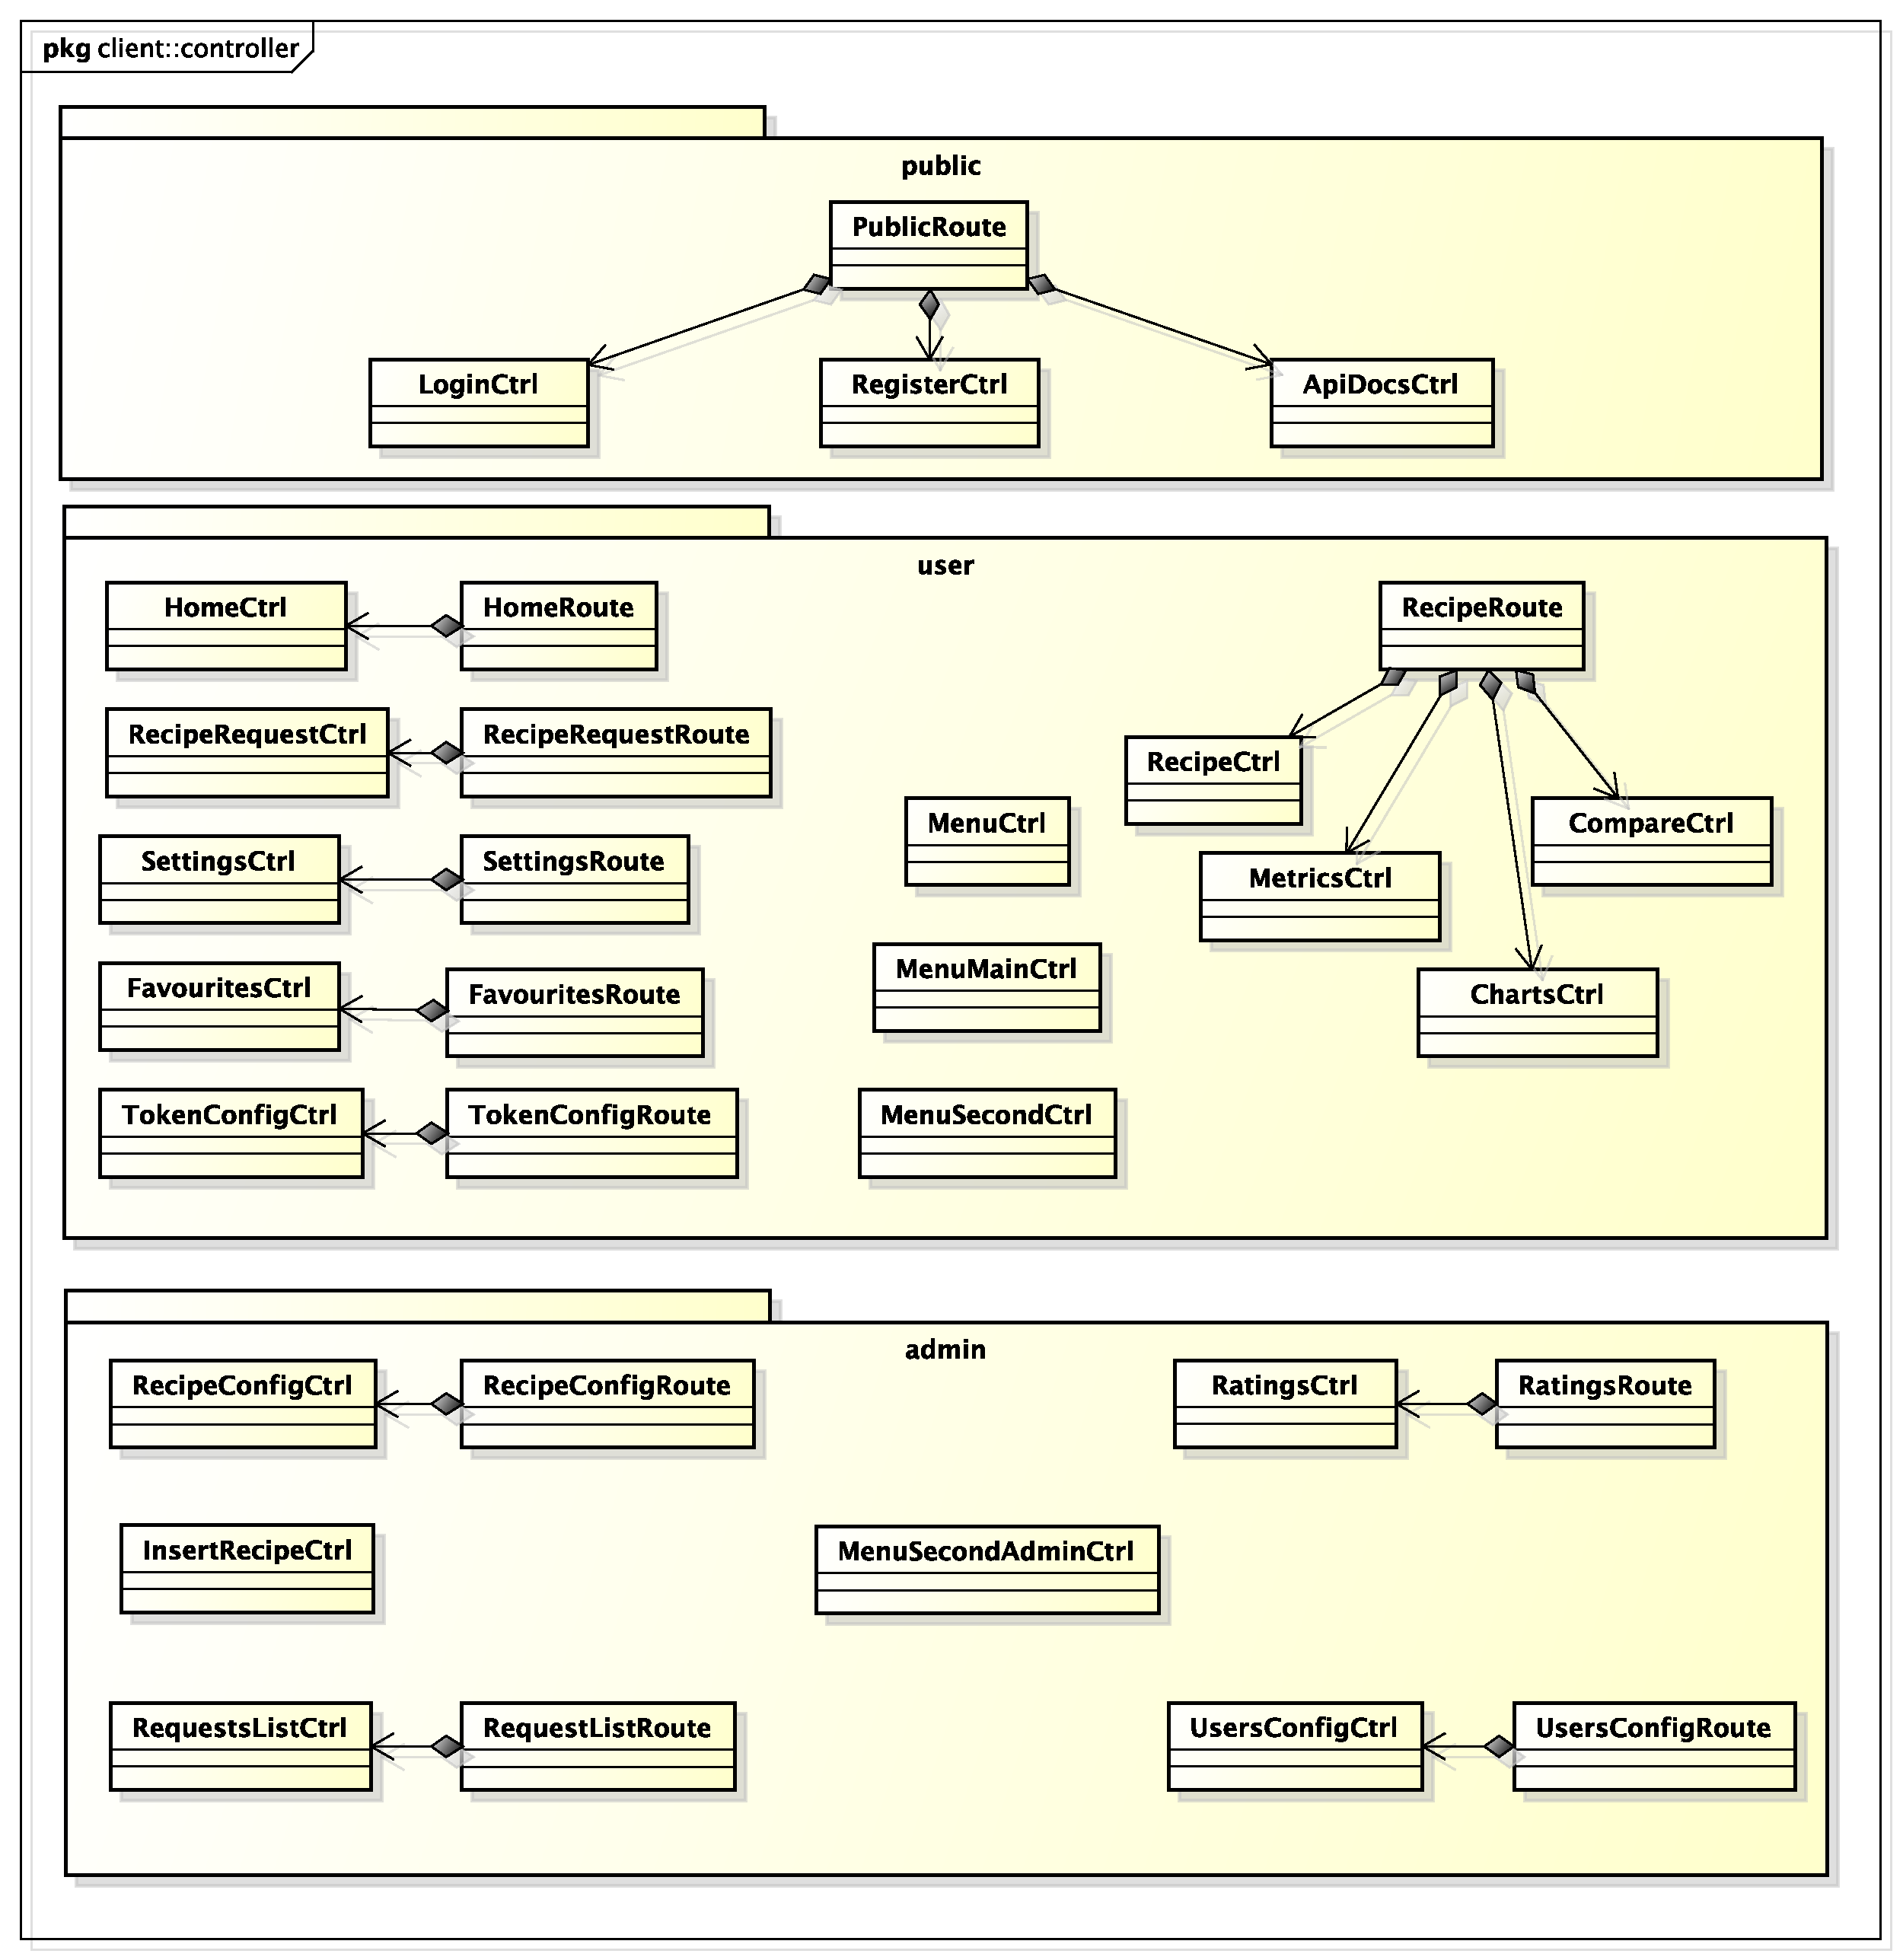
\includegraphics[scale=0.4]{./images/client_controller.pdf}}
	\caption{Package - client::controller}
\end{figure}

\begin{itemize}
	\item \textbf{Descrizione}: è il package che contiene le componenti che contengono i controller dell'applicazione e che incapsulano le funzionalità di two-way data binding tra le View e il Model. In esse è contenuta la logica applicativa riguardante le diverse pagine HTML;
	\item \textbf{Padre}: client;
	\item \textbf{Package contenuti}:
		\begin{itemize}
			\item client::controller::public
			\item client::controller::user
			\item client::controller::admin
		\end{itemize}
\end{itemize}
% subsubsection bdsm_app_client_controller (end)


\subsubsection{bdsm\_app::client::controller::public} % (fold)
\label{ssub:bdsm_app_client_controller_public}
\begin{figure}[htbp]
	\centering
	\centerline{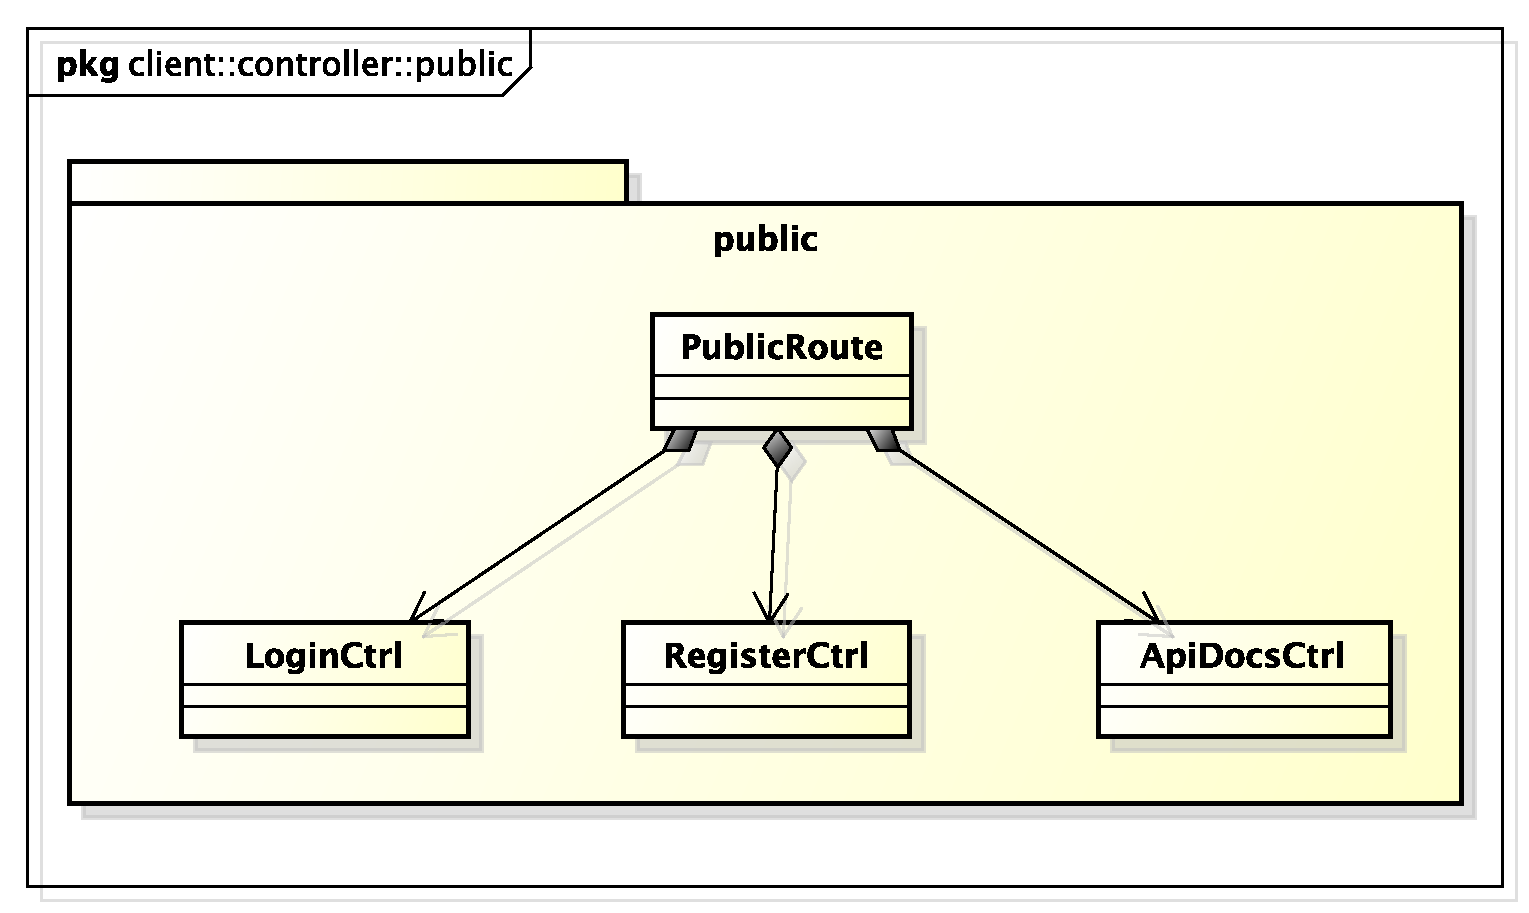
\includegraphics[scale=0.6]{./images/client_controller_public.pdf}}
	\caption{Package - client::controller::public}
\end{figure}

\begin{itemize}
	\item \textbf{Descrizione}: è il package che contiene le classi che controllano le decisioni di che pagine HTML mostrare all'utente che non si è ancora autenticato e di quali operazioni poter effettuare su di esse;
	\item \textbf{Padre}: client::controller
	\item \textbf{Interazione con altri componenti}:
		\begin{itemize}
			\item client::model::public
			\item client::view::public
		\end{itemize}
\end{itemize}

	\paragraph{Classi} % (fold)
		\subparagraph{bdsm\_app::client::controller::public::PublicRoute} % (fold)
		\label{subp:bdsm_app_client_controller_public_publicrouteconfig}
		\begin{itemize}
			\item \textbf{Descrizione}: la classe serve a gestire l'indirizzamento e l'assegnazione di uno stato al template HTML riguardante le pagine che può visualizzare un utente non autenticato, quali quella di autenticazione, di registrazione o di visione della documentazione dei servizi REST offerti;
			\item \textbf{Utilizzo}: viene utilizzata per reindirizzare l'utente al template HTML adeguato in caso si voglia o autenticare o registrare al sistema, o visualizzare i servizi REST offerti, ed assegnare al template scelto il controller opportuno per gestire i diversi compiti. Nel caso l'utente fosse già autenticato, la classe provvederà a reindirizzarlo all'URL associato alla Home;
			\item \textbf{Relazioni con altre classi}:
				\begin{itemize}
					\item client::view::public::Login
					\item client::view::public::Register
					\item client::view::public::ApiDocs
					\item client::controller::public::LoginCtrl
					\item client::controller::public::RegisterCtrl
				\end{itemize}
		\end{itemize}
		% subparagraph bdsm_app_client_controller_public_publicrouteconfig (end)

		\subparagraph{bdsm\_app::client::controller::public::LoginCtrl} % (fold)
		\label{subp:bdsm_app_client_controller_public_loginctrl}
			\begin{itemize}
				\item \textbf{Descrizione}: la classe è il controller che serve a gestire l'autenticazione al sistema;
				\item \textbf{Utilizzo}: viene utilizzata per gestire le operazioni di autenticazione al sistema qualora un utente non autenticato decidesse di effettuare l'accesso. Richiamando quindi i servizi che mettono in comunicazione il client con il server, verifica le credenziali ed effettua un reindirizzamento alla Home qualora fossero valide;
				\item \textbf{Relazioni con altre classi}:
					\begin{itemize}
						\item [TO DO]
						\item client::view::public::Login
						\item client::controller::public::PublicRoute
					\end{itemize}
			\end{itemize}
		% subparagraph bdsm_app_client_controller_public_loginctrl (end)

		\subparagraph{bdsm\_app::client::controller::public::RegisterCtrl} % (fold)
		\label{subp:bdsm_app_client_controller_public_registerctrl}
			\begin{itemize}
				\item \textbf{Descrizione}: la classe è il controller che serve a gestire la registrazione al sistema;
				\item \textbf{Utilizzo}: viene utilizzata per gestire le operazioni di registrazione al sistema qualora un utente che non si è ancora registrato decidesse di effettuare l'accesso. Richiamando quindi i servizi che mettono in comunicazione il client con il server, verifica le credenziali ed effettua un reindirizzamento alla pagina di Login qualora la registrazione fosse avvenuta con successo;
				\item \textbf{Relazioni con altre classi}:
					\begin{itemize}
						\item [TO DO]
						\item client::view::public::Register
						\item client::controller::public::PublicRoute
					\end{itemize}
			\end{itemize}
		% subparagraph bdsm_app_client_controller_public_registerctrl (end)

		\subparagraph{bdsm\_app::client::controller::public::ApiDocsCtrl} % (fold)
		\label{subp:bdsm_app_client_controller_public_apidocsctrl}
		[TO DO] (non so se necessario, se la cosa è statica non servirebbe)
		% subparagraph bdsm_app_client_controller_public_apidocsctrl (end)


% subsubsection bdsm_app_client_controller_public (end)



\subsubsection{bdsm\_app::client::controller::user} % (fold)
\label{ssub:bdsm_app_client_controller_user}
\begin{figure}[htbp]
	\centering
	\centerline{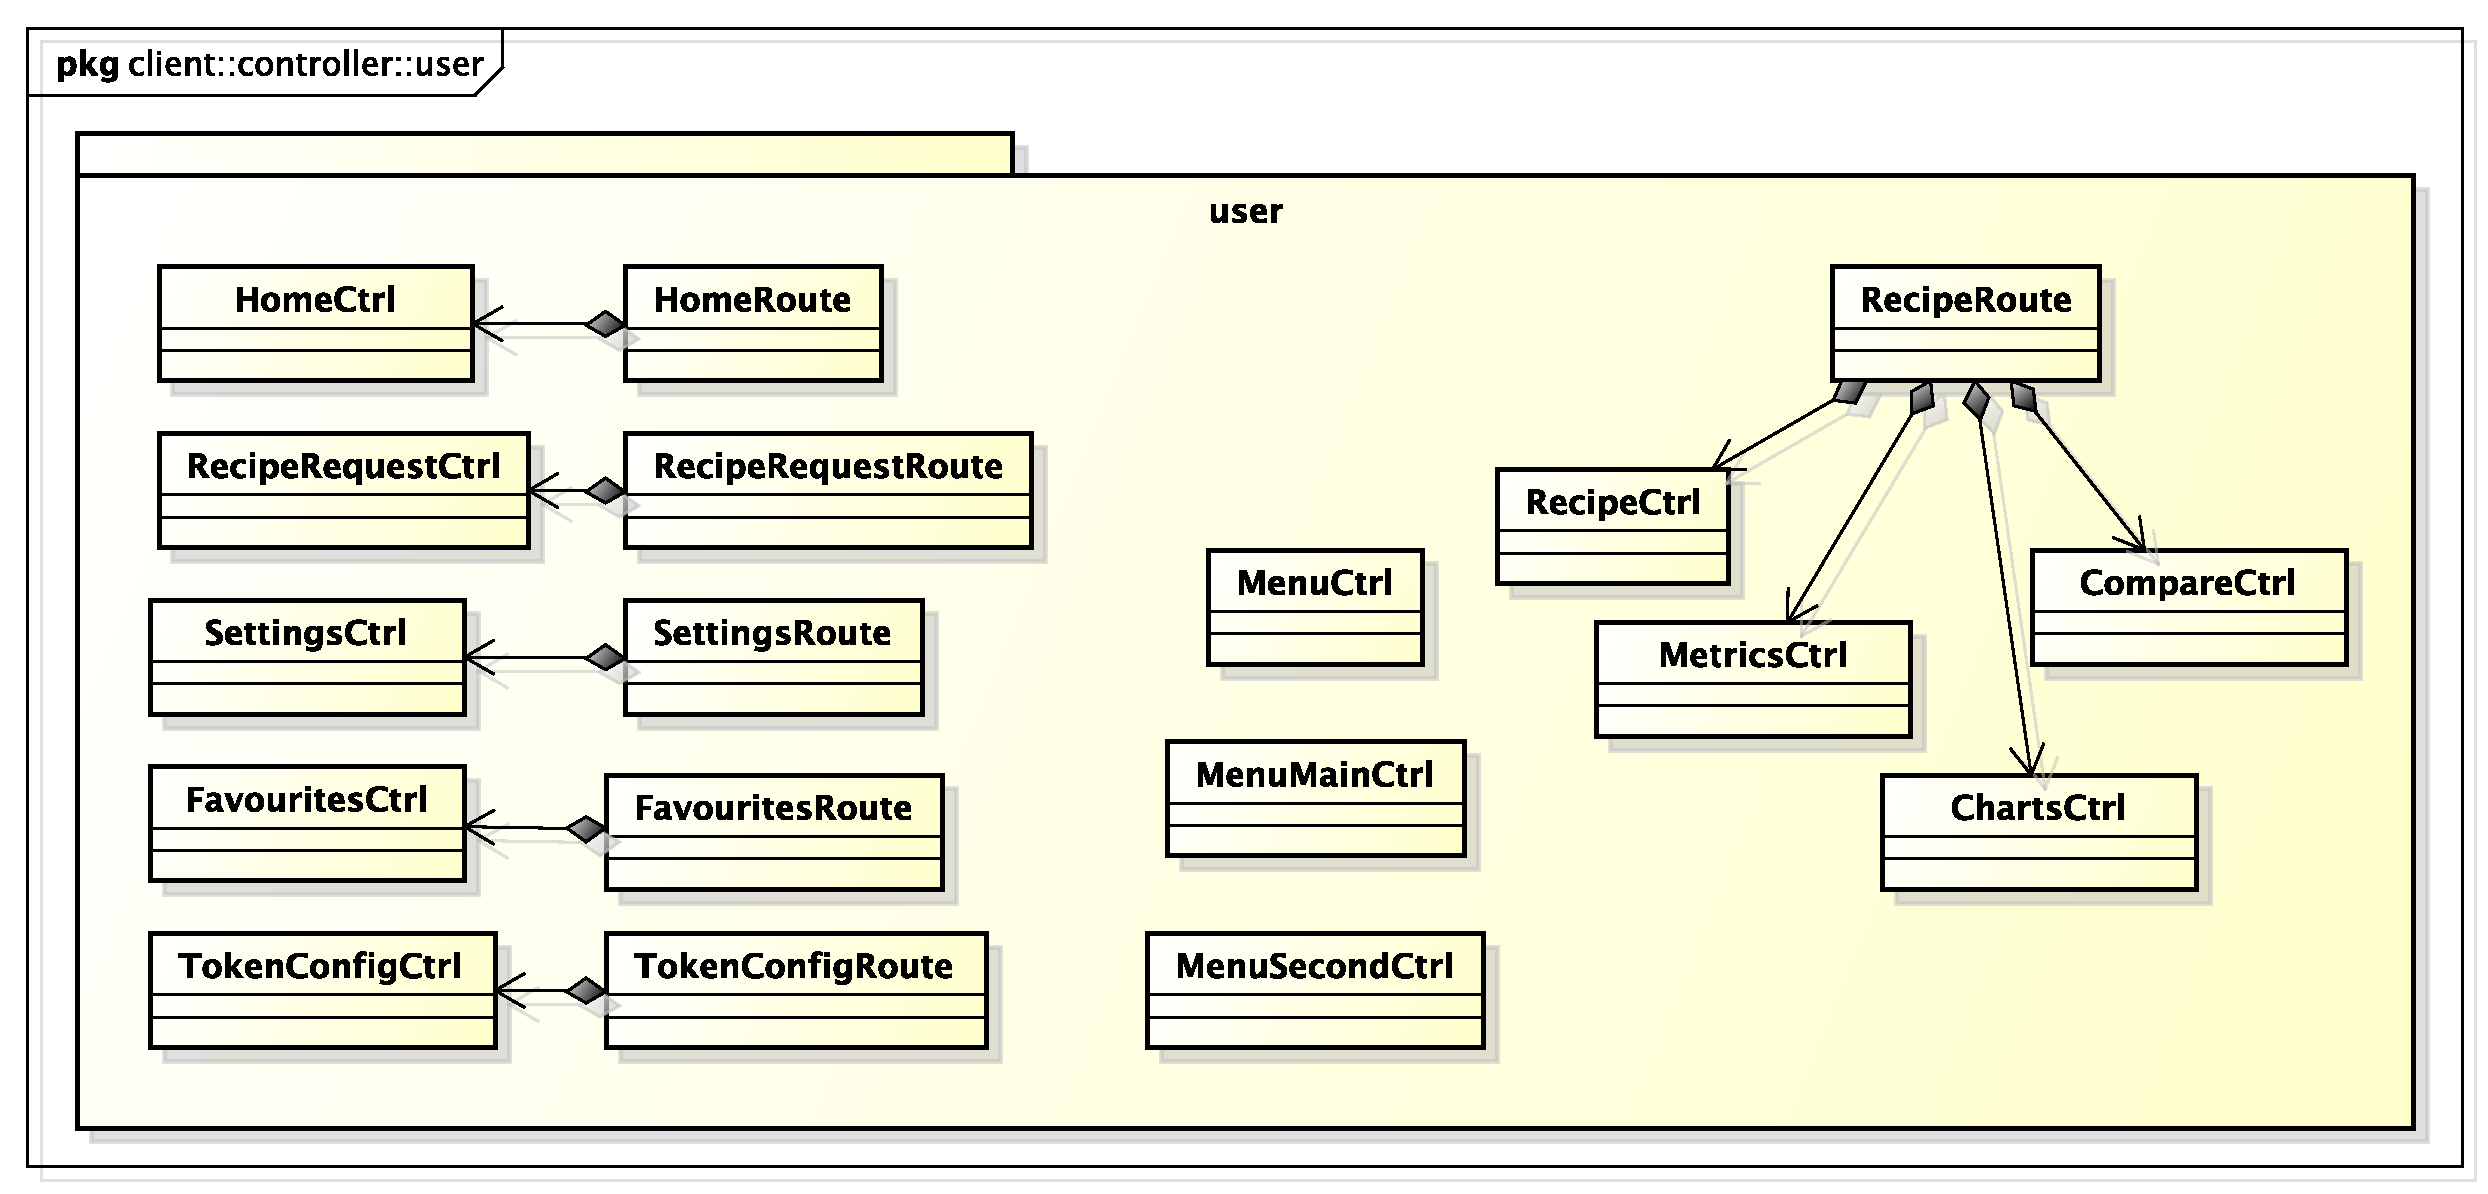
\includegraphics[scale=0.45]{./images/client_controller_user.pdf}}
	\caption{Package - client::controller::user}
\end{figure}

\begin{itemize}
	\item \textbf{Descrizione}: è il package che contiene le classi che controllano le decisioni di che pagine HTML mostrare all'utente autenticato e di quali operazioni poter effettuare su di esse;
	\item \textbf{Padre}: client::controller
	\item \textbf{Interazione con altri componenti}:
		\begin{itemize}
			\item client::model::user
			\item client::view::user
		\end{itemize}
\end{itemize}

	\paragraph{Classi} % (fold)
		\subparagraph{bdsm\_app::client::controller::user::MenuCtrl} % (fold)
		\label{subp:client_controller_user_menuctrl}
			\begin{itemize}
				\item \textbf{Descrizione}: [TO DO];
				\item \textbf{Utilizzo}: [TO DO];
				\item \textbf{Classi ereditate}: [TO DO];
				\item \textbf{Relazioni con altre classi}: [TO DO].
			\end{itemize}
		% subparagraph client_controller_user_menuctrl (end)

		\subparagraph{bdsm\_app::client::controller::user::MenuMainCtrl} % (fold)
		\label{subp:client_controller_user_menumainctrl}
			\begin{itemize}
				\item \textbf{Descrizione}: [TO DO];
				\item \textbf{Utilizzo}: [TO DO];
				\item \textbf{Classi ereditate}: [TO DO];
				\item \textbf{Relazioni con altre classi}: [TO DO].
			\end{itemize}
		% subparagraph client_controller_user_menumainctrl (end)

		\subparagraph{bdsm\_app::client::controller::user::MenuSecondCtrl} % (fold)
		\label{subp:client_controller_user_menusecondctrl}
			\begin{itemize}
				\item \textbf{Descrizione}: [TO DO];
				\item \textbf{Utilizzo}: [TO DO];
				\item \textbf{Classi ereditate}: [TO DO];
				\item \textbf{Relazioni con altre classi}: [TO DO].
			\end{itemize}
		% subparagraph client_controller_user_menusecondctrl (end)

		\subparagraph{bdsm\_app::client::controller::user::HomeRoute} % (fold)
		\label{subp:bdsm_app_client_controller_user_homerouteconfig}
			\begin{itemize}
				\item \textbf{Descrizione}: [TO DO];
				\item \textbf{Utilizzo}: [TO DO];
				\item \textbf{Classi ereditate}: [TO DO];
				\item \textbf{Relazioni con altre classi}: [TO DO].
			\end{itemize}
		% subparagraph bdsm_app_client_controller_user_homerouteconfig (end)

		\subparagraph{bdsm\_app::client::controller::user::HomeCtrl} % (fold)
		\label{subp:client_controller_user_homectrl}
			\begin{itemize}
				\item \textbf{Descrizione}: [TO DO];
				\item \textbf{Utilizzo}: [TO DO];
				\item \textbf{Classi ereditate}: [TO DO];
				\item \textbf{Relazioni con altre classi}: [TO DO].
			\end{itemize}
		% subparagraph client_controller_user_homectrl (end)

		\subparagraph{bdsm\_app::client::controller::user::RecipeRoute} % (fold)
		\label{subp:bdsm_app_client_controller_user_reciperouteconfig}
			\begin{itemize}
				\item \textbf{Descrizione}: [TO DO];
				\item \textbf{Utilizzo}: [TO DO];
				\item \textbf{Classi ereditate}: [TO DO];
				\item \textbf{Relazioni con altre classi}: [TO DO].
			\end{itemize}
		% subparagraph bdsm_app_client_controller_user_reciperouteconfig (end)

		\subparagraph{bdsm\_app::client::controller::user::RecipeCtrl} % (fold)
		\label{subp:client_controller_user_recipectrl}
			\begin{itemize}
				\item \textbf{Descrizione}: [TO DO];
				\item \textbf{Utilizzo}: [TO DO];
				\item \textbf{Classi ereditate}: [TO DO];
				\item \textbf{Relazioni con altre classi}: [TO DO].
			\end{itemize}
		% subparagraph client_controller_user_recipectrl (end)

		\subparagraph{bdsm\_app::client::controller::user:.MetricsCtrl} % (fold)
		\label{subp:client_controller_user_metricsctrl}
			\begin{itemize}
				\item \textbf{Descrizione}: [TO DO];
				\item \textbf{Utilizzo}: [TO DO];
				\item \textbf{Classi ereditate}: [TO DO];
				\item \textbf{Relazioni con altre classi}: [TO DO].
			\end{itemize}
		% subparagraph client_controller_user_metricsctrl (end)

		\subparagraph{bdsm\_app::client::controller::user::ChartsCtrl} % (fold)
		\label{subp:client_controller_user_chartsctrl}
			\begin{itemize}
				\item \textbf{Descrizione}: [TO DO];
				\item \textbf{Utilizzo}: [TO DO];
				\item \textbf{Classi ereditate}: [TO DO];
				\item \textbf{Relazioni con altre classi}: [TO DO].
			\end{itemize}
		% subparagraph client_controller_user_chartsctrl (end)

		\subparagraph{bdsm\_app::client::controller::user::CompareCtrl} % (fold)
		\label{subp:client_controller_user_comparectrl}
			\begin{itemize}
				\item \textbf{Descrizione}: [TO DO];
				\item \textbf{Utilizzo}: [TO DO];
				\item \textbf{Classi ereditate}: [TO DO];
				\item \textbf{Relazioni con altre classi}: [TO DO].
			\end{itemize}
		% subparagraph client_controller_user_comparectrl (end)

		\subparagraph{bdsm\_app::client::controller::user::RecipeRequestRoute} % (fold)
		\label{subp:bdsm_app_client_controller_user_reciperequestrouteconfig}
			\begin{itemize}
				\item \textbf{Descrizione}: [TO DO];
				\item \textbf{Utilizzo}: [TO DO];
				\item \textbf{Classi ereditate}: [TO DO];
				\item \textbf{Relazioni con altre classi}: [TO DO].
			\end{itemize}
		% subparagraph bdsm_app_client_controller_user_reciperequestrouteconfig (end)

		\subparagraph{bdsm\_app::client::controller::user::RecipeRequestCtrl} % (fold)
		\label{subp:client_controller_user_reciperequestctrl}
			\begin{itemize}
				\item \textbf{Descrizione}: [TO DO];
				\item \textbf{Utilizzo}: [TO DO];
				\item \textbf{Classi ereditate}: [TO DO];
				\item \textbf{Relazioni con altre classi}: [TO DO].
			\end{itemize}
		% subparagraph client_controller_user_reciperequestctrl (end)

		\subparagraph{bdsm\_app::client::controller::user::FavouritesRoute} % (fold)
		\label{subp:bdsm_app_client_controller_user_favouritesroute}
			\begin{itemize}
				\item \textbf{Descrizione}: [TO DO];
				\item \textbf{Utilizzo}: [TO DO];
				\item \textbf{Classi ereditate}: [TO DO];
				\item \textbf{Relazioni con altre classi}: [TO DO].
			\end{itemize}
		% subparagraph bdsm_app_client_controller_user_favouritesroute (end)

		\subparagraph{bdsm\_app::client::controller::user::FavouritesCtrl} % (fold)
		\label{subp:client_controller_user_favouritesctrl}
			\begin{itemize}
				\item \textbf{Descrizione}: [TO DO];
				\item \textbf{Utilizzo}: [TO DO];
				\item \textbf{Classi ereditate}: [TO DO];
				\item \textbf{Relazioni con altre classi}: [TO DO].
			\end{itemize}
		% subparagraph client_controller_user_favouritesctrl (end)

		\subparagraph{bdsm\_app::client::controller::user::TokenConfigRoute} % (fold)
		\label{subp:bdsm_app_client_controller_user_tokenconfigroute}
			\begin{itemize}
				\item \textbf{Descrizione}: [TO DO];
				\item \textbf{Utilizzo}: [TO DO];
				\item \textbf{Classi ereditate}: [TO DO];
				\item \textbf{Relazioni con altre classi}: [TO DO].
			\end{itemize}
		% subparagraph bdsm_app_client_controller_user_tokenconfigroute (end)

		\subparagraph{bdsm\_app::client::controller::user::TokenConfigCtrl} % (fold)
		\label{subp:client_controller_user_tokenconfigctrl}
			\begin{itemize}
				\item \textbf{Descrizione}: [TO DO];
				\item \textbf{Utilizzo}: [TO DO];
				\item \textbf{Classi ereditate}: [TO DO];
				\item \textbf{Relazioni con altre classi}: [TO DO].
			\end{itemize}
		% subparagraph client_controller_user_tokenconfigctrl (end)

		\subparagraph{bdsm\_app::client::controller::user::SettingsRoute} % (fold)
		\label{subp:bdsm_app_client_controller_user_settingsroute}
			\begin{itemize}
				\item \textbf{Descrizione}: [TO DO];
				\item \textbf{Utilizzo}: [TO DO];
				\item \textbf{Classi ereditate}: [TO DO];
				\item \textbf{Relazioni con altre classi}: [TO DO].
			\end{itemize}
		% subparagraph bdsm_app_client_controller_user_settingsroute (end)

		\subparagraph{bdsm\_app::client::controller::user::SettingsCtrl} % (fold)
		\label{subp:client_controller_user_settingsctrl}
			\begin{itemize}
				\item \textbf{Descrizione}: [TO DO];
				\item \textbf{Utilizzo}: [TO DO];
				\item \textbf{Classi ereditate}: [TO DO];
				\item \textbf{Relazioni con altre classi}: [TO DO].
			\end{itemize}
		% subparagraph client_controller_user_settingsctrl (end)

		\subparagraph{bdsm\_app::client::controller::user::LogoutCtrl} % (fold)
		\label{subp:bdsm_app_client_controller_user_logoutctrl}
			\begin{itemize}
				\item \textbf{Descrizione}: [TO DO];
				\item \textbf{Utilizzo}: [TO DO];
				\item \textbf{Classi ereditate}: [TO DO];
				\item \textbf{Relazioni con altre classi}: [TO DO].
			\end{itemize}
		% subparagraph bdsm_app_client_controller_user_logoutctrl (end)

% subsubsection bdsm_app_client_controller_user (end)






\subsubsection{bdsm\_app::client::controller::admin} % (fold)
\label{ssub:bdsm_app_client_controller_admin}
\begin{figure}[htbp]
	\centering
	\centerline{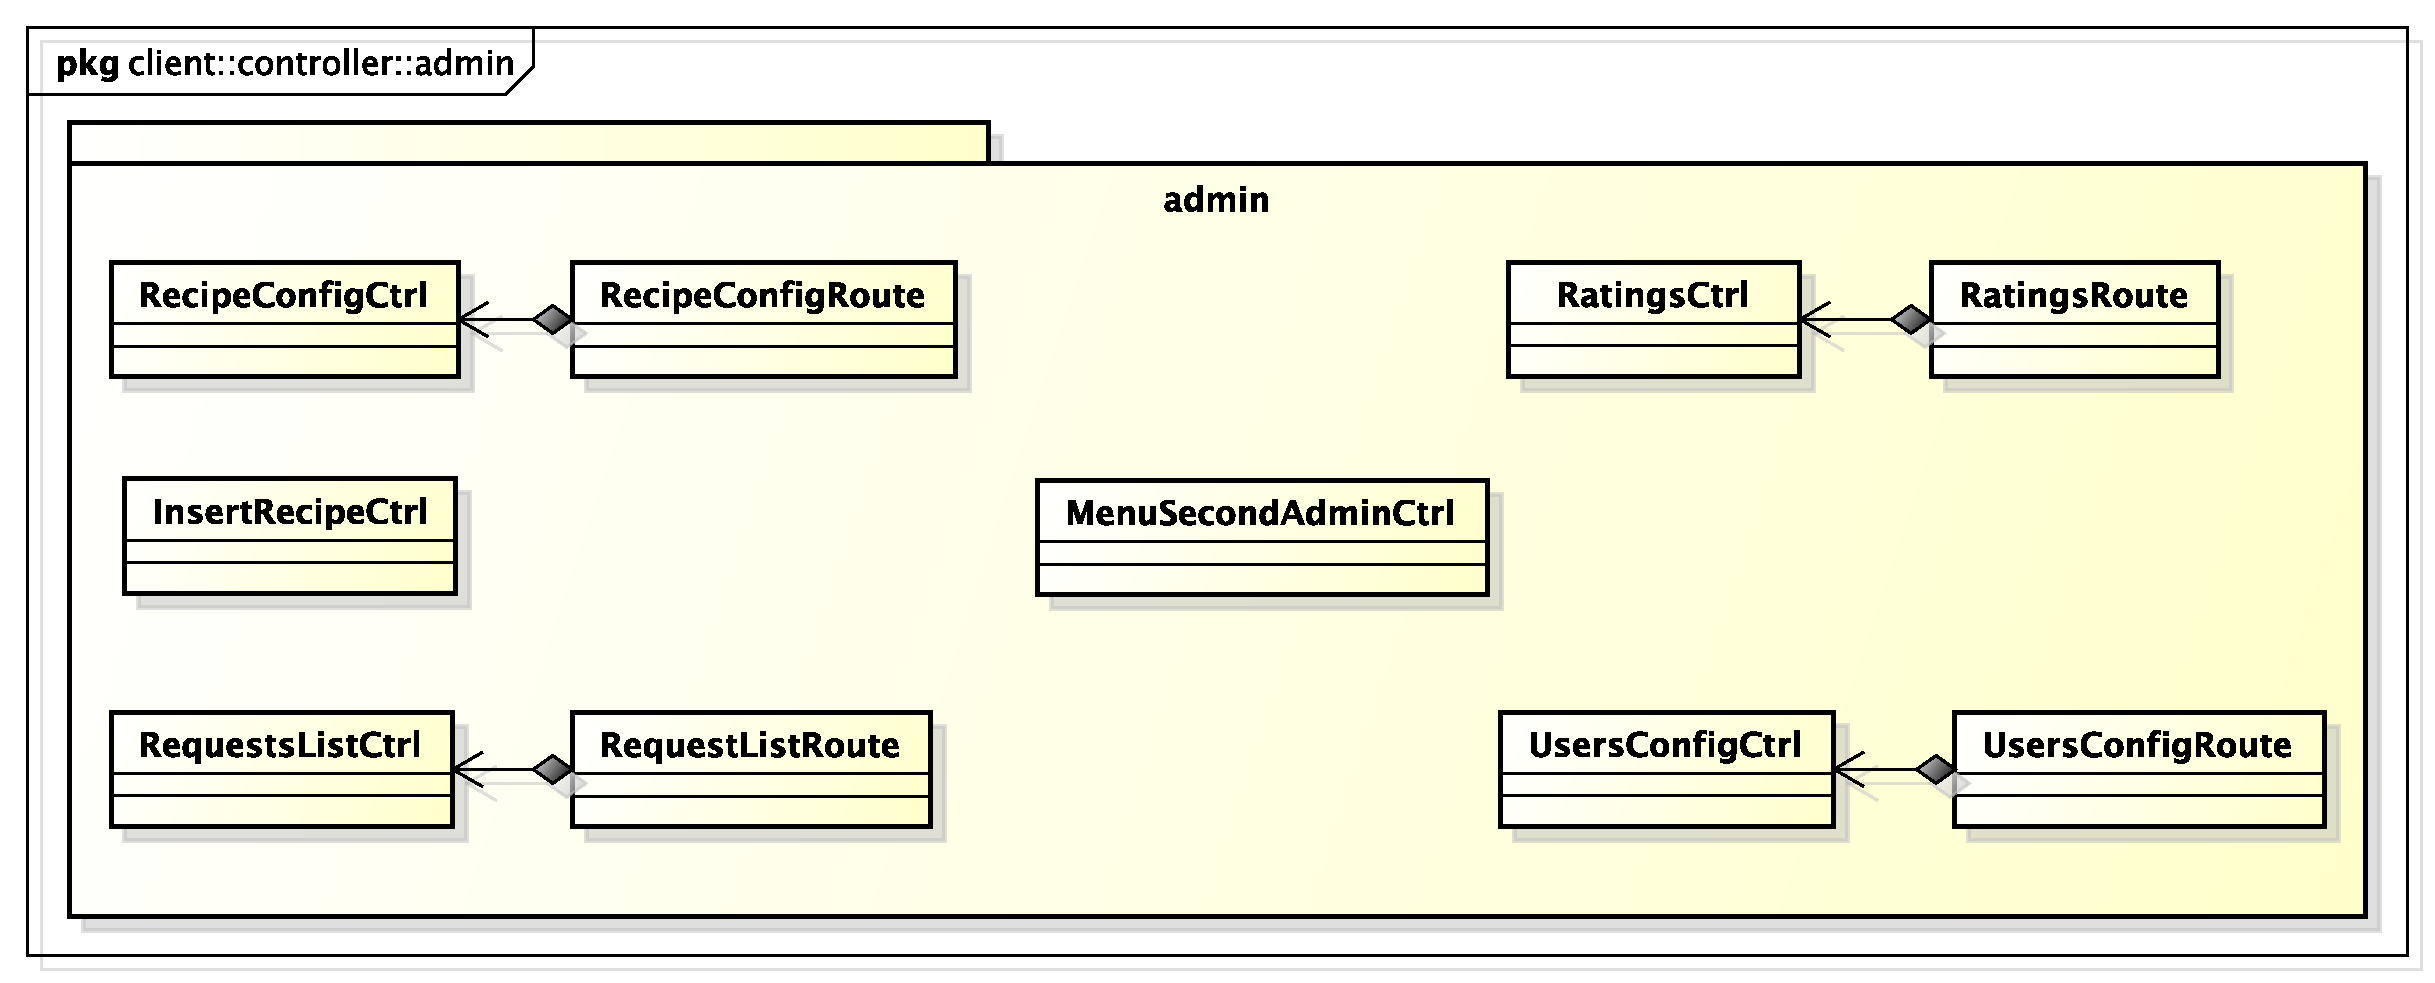
\includegraphics[scale=0.45]{./images/client_controller_admin.pdf}}
	\caption{Package - client::controller::admin}
\end{figure}

\begin{itemize}
	\item \textbf{Descrizione}: è il package che contiene le classi che controllano le decisioni di che pagine HTML mostrare all'amministratore e di quali operazioni poter effettuare su di esse;
	\item \textbf{Padre}: client::controller
	\item \textbf{Interazione con altri componenti}:
		\begin{itemize}
			\item client::model::admin
			\item client::view::admin
		\end{itemize}
\end{itemize}

	\paragraph{Classi} % (fold)
		\subparagraph{bdsm\_app::client::controller::admin::MenuSecondAdminCtrl} % (fold)
		\label{subp:bdsm_app_client_controller_admin_menusecondadminctrl}
			\begin{itemize}
				\item \textbf{Descrizione}: [TO DO];
				\item \textbf{Utilizzo}: [TO DO];
				\item \textbf{Classi ereditate}: [TO DO];
				\item \textbf{Relazioni con altre classi}: [TO DO].
			\end{itemize}
		% subparagraph bdsm_app_client_controller_admin_menusecondadminctrl (end)

		\subparagraph{bdsm\_app::client::controller::admin::RecipeConfigRoute} % (fold)
		\label{subp:bdsm_app_client_controller_admin_recipeconfigroute}
			\begin{itemize}
				\item \textbf{Descrizione}: [TO DO];
				\item \textbf{Utilizzo}: [TO DO];
				\item \textbf{Classi ereditate}: [TO DO];
				\item \textbf{Relazioni con altre classi}: [TO DO].
			\end{itemize}
		% subparagraph bdsm_app_client_controller_admin_recipeconfigroute (end)

		\subparagraph{bdsm\_app::client::controller::admin::RecipeConfigCtrl} % (fold)
		\label{subp:bdsm_app_client_controller_admin_recipeconfigctrl}
			\begin{itemize}
				\item \textbf{Descrizione}: [TO DO];
				\item \textbf{Utilizzo}: [TO DO];
				\item \textbf{Classi ereditate}: [TO DO];
				\item \textbf{Relazioni con altre classi}: [TO DO].
			\end{itemize}
		% subparagraph bdsm_app_client_controller_admin_recipeconfigctrl (end)

		\subparagraph{bdsm\_app::client::controller::admin::RequestListRoute} % (fold)
		\label{subp:bdsm_app_client_controller_admin_recipelistroute}
			\begin{itemize}
				\item \textbf{Descrizione}: [TO DO];
				\item \textbf{Utilizzo}: [TO DO];
				\item \textbf{Classi ereditate}: [TO DO];
				\item \textbf{Relazioni con altre classi}: [TO DO].
			\end{itemize}
		% subparagraph bdsm_app_client_controller_admin_recipelistroute (end)

		\subparagraph{bdsm\_app::client::controller::admin::RequestListCtrl} % (fold)
		\label{subp:bdsm_app_client_controller_admin_requestlistctrl}
			\begin{itemize}
				\item \textbf{Descrizione}: [TO DO];
				\item \textbf{Utilizzo}: [TO DO];
				\item \textbf{Classi ereditate}: [TO DO];
				\item \textbf{Relazioni con altre classi}: [TO DO].
			\end{itemize}
		% subparagraph bdsm_app_client_controller_admin_requestlistctrl (end)

		\subparagraph{bdsm\_app::client::controller::admin::InsertRecipeCtrl} % (fold)
		\label{subp:bdsm_app_client_controller_admin_insertctrl}
			\begin{itemize}
				\item \textbf{Descrizione}: [TO DO];
				\item \textbf{Utilizzo}: [TO DO];
				\item \textbf{Classi ereditate}: [TO DO];
				\item \textbf{Relazioni con altre classi}: [TO DO].
			\end{itemize}
		% subparagraph bdsm_app_client_controller_admin_insertctrl (end)

		\subparagraph{bdsm\_app::client::controller::admin::RatingsRoute} % (fold)
		\label{subp:bdsm_app_client_controller_admin_ratingsroute}
			\begin{itemize}
				\item \textbf{Descrizione}: [TO DO];
				\item \textbf{Utilizzo}: [TO DO];
				\item \textbf{Classi ereditate}: [TO DO];
				\item \textbf{Relazioni con altre classi}: [TO DO].
			\end{itemize}
		% subparagraph bdsm_app_client_controller_admin_ratingsroute (end)

		\subparagraph{bdsm\_app::client::controller::admin::RatingsCtrl} % (fold)
		\label{subp:bdsm_app_client_controller_admin_ratingsctrl}
			\begin{itemize}
				\item \textbf{Descrizione}: [TO DO];
				\item \textbf{Utilizzo}: [TO DO];
				\item \textbf{Classi ereditate}: [TO DO];
				\item \textbf{Relazioni con altre classi}: [TO DO].
			\end{itemize}
		% subparagraph bdsm_app_client_controller_admin_ratingsctrl (end)

		\subparagraph{bdsm\_app::client::controller::admin::UserConfigRoute} % (fold)
		\label{subp:bdsm_app_client_controller_admin_userconfigroute}
		
		% subparagraph bdsm_app_client_controller_admin_userconfigroute (end)

		\subparagraph{bdsm\_app::client::controller::admin::UserConfigCtrl} % (fold)
		\label{subp:bdsm_app_client_controller_admin_userconfigctrl}
			\begin{itemize}
				\item \textbf{Descrizione}: [TO DO];
				\item \textbf{Utilizzo}: [TO DO];
				\item \textbf{Classi ereditate}: [TO DO];
				\item \textbf{Relazioni con altre classi}: [TO DO].
			\end{itemize}
		% subparagraph bdsm_app_client_controller_admin_userconfigctrl (end)


% subsubsection bdsm_app_client_controller_admin (end)